\chapter{Importance Sampling}
There are two different ways to think about importance sampling.
The more traditional one is to go back to the primary problem that
Monte Carlo  wants to solve,
namely to approximate the value of an expectation
$\mu = \int \phi_0(x)dF_0(x) $ for some function $\phi_0$ and some CDF $F_0$.
However, $(\phi_0,F_0)$ is not the only pair $(\phi,F)$ for which
$\int \phi(x)dF(x) $ equals the specific number $\mu$. Indeed, given any other
CDF $F_1$,
\begin{align*}
	\mu & = \int \phi_0(x)dF_0(x)                      \\
	    & = \int \phi_0(x)\frac{dF_0}{dF_1}(x) dF_1(x) \\
	    & = \int \lambda(x)\phi_0(x)dF_1(x).
\end{align*}

where $\lambda(x)=\frac{dF_0}{dF_1}(x)$. If $F_0$, $F_1$ have densities
$f_0$, $f_1$, then $\lambda(x)=\frac{f_0(x)}{f_1(x)}$; if $F_0,$ $F_1$
have respective pmfs $f_0$, $f_1$, then also $\lambda(x)=\frac{f_0(x)}{f_1(x)}$
This raises the interesting possibility that we can sample from a general $F_1$, and
subsequently use the usual Monte Carlo estimate
\[
	\hat{\mu} = \frac{1}{n} \sum_{i = 1}^{n} \lambda(X_i)\phi_0(X_i) = E_{F_1}[\lambda(X_i)\phi_0(X_i)].
\]

where $X_1, X_2, \ldots, X_n$ is Monte Carlo sample from $F_1$.
Importance sampling poses the problem of finding an optimal choice of $F_1$ for which to sample,
so that $\hat{\mu}$ has the smallest possible variance.
The distribution $F_1$ hat ultimately gets
chosen is called the \textit{importance sampling distribution}.

We can visualize this method by an example.

\begin{example}
	Suppose we want to evaluate
	\[
		I = \int_{0}^{10} e^{-2 |x-5|} dx.
	\]
	doing it analytically we get $I = 0.9999$.

	Now, suppose $h(x) = e^{-2 |x-5|}$ then we want to evaluate
	\[
		I = \int_{0}^{10} h(x) dx
	\]
	Now,
	\begin{align*}
		\label{hx with U}
		I & = \int_{0}^{10} h(x) dx                                                                                                            \\
		  & = \int_{0}^{10} h(x)\frac{10}{10} dx                                                                                               \\
		  & = \int_{0}^{10} 10 \times h(x) \frac{1}{10} dx = \int_{0}^{10} 10h(x) p(x) dx \text{ where } p(x)\text{ pdf of }U(0,1) \numberthis \\
		  & = E_U[10 \times h(U)] \text{ where, }  U\sim U(0,10).
	\end{align*}

	By Ordinary Monte Carlo technique we can estimate $I$ by $\frac{1}{N}\sum_{i = 1}^{N} 10 \times h(U_i)$ where $U_i\sim U(0,10)$ for $i=1,2,\ldots,N$
	for the large number of $N$.
	\begin{figure}[H]
		\centering
		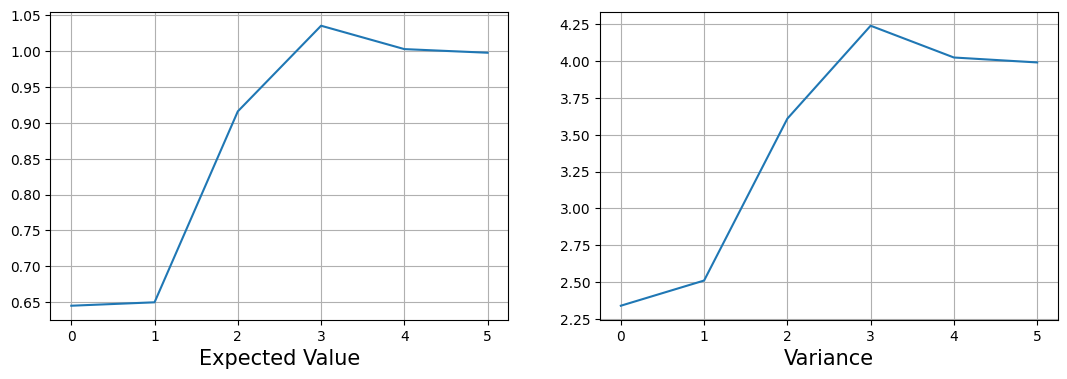
\includegraphics[width=0.8\textwidth]{int_h(x)_MC.png}
		\caption{Monte Carlo integration of $\int_{0}^{10} e^{-2 |x-5|} dx$.}
		\label{MC:IntegrationOFe-2|x*5|}
	\end{figure}
	\begin{table}[h]
		\centering
		\begin{tabular}{lcc}
			\hline
			Sample Size & Estimated Value I=0.9999 & Variance \\
			\hline
			10          & 2.3243                   & 5.6912   \\
			100         & 1.0372                   & 3.6717   \\
			1000        & 0.8871                   & 3.5543   \\
			10000       & 1.0467                   & 4.2416   \\
			100000      & 1.0053                   & 4.0089   \\
			1000000     & 1.0054                   & 4.0346   \\
			\hline
		\end{tabular}
		\caption{Monte Carlo integration of $\int_{0}^{10} e^{-2 |x-5|} dx$.}
		\label{tab:IntegrationOFe-2|x*5|}
	\end{table}
	Here we can see that for sample size 1M we get a pretty good estimation of $I$ with less then $0.6\%$ error but the variance is very high.
	If we see at left of Figure (\ref{fig:hxwithU01andN01}) we can see we are taking unnecessary value from low frequency part of $h(x)$ that is,
	from extream left and right. If we choose an importance sampling distribution that has similar curve as $h(x)$ then we can estimate $I$ with low variance.
	If we choose importance sampling distribution as $N(5,1)$ then we see from right of Figure (\ref{fig:hxwithU01andN01}) it has similar pattern as $h(x)$.
	\begin{figure}[H]
		\centering
		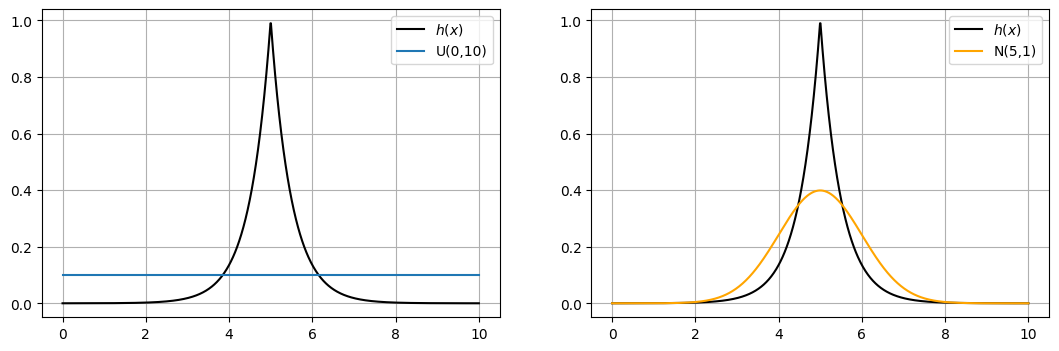
\includegraphics[width=0.8\textwidth]{h(x)_with_normal_and_uniform.png}
		\caption{$h(x)$ with $U(0,1)$ and $N(5,1)$}
		\label{fig:hxwithU01andN01}
	\end{figure}

	Let, $q(x)$ is pdf of $N(0,1)$ then, from (\ref{hx with U})
	\begin{align*}
		I & = \int_{0}^{10} 10h(x) p(x) dx                                            \\
		  & = \int_{0}^{10} 10 h(x) \frac{p(x)}{q(x)} q(x)dx                          \\
		  & = E_X\left[ 10 h(X) \frac{p(X)}{q(X)} \right] \text{ where } X\sim N(5,1) \\
		  & = E_X\left[ 10 h(X) \lambda(X) \right]\text{ where } X\sim N(5,1)
	\end{align*}
	Where, $\lambda(x) = \frac{p(X)}{q(X)}$ here $p(x)$ is pdf of $U(0,1)$ and $q(x)$ is pdf of $N(5,1)$. Now using usual Monte Carlo estimate
	\[
		I = \frac{1}{N} \sum_{i = 1}^{N} 10 h(X_i) \lambda(X_i)
	\]
	where $X_1, X_2,\ldots,X_N$ is Monte Carlo sample from $N(5,1)$.
	\begin{figure}[H]
		\centering
		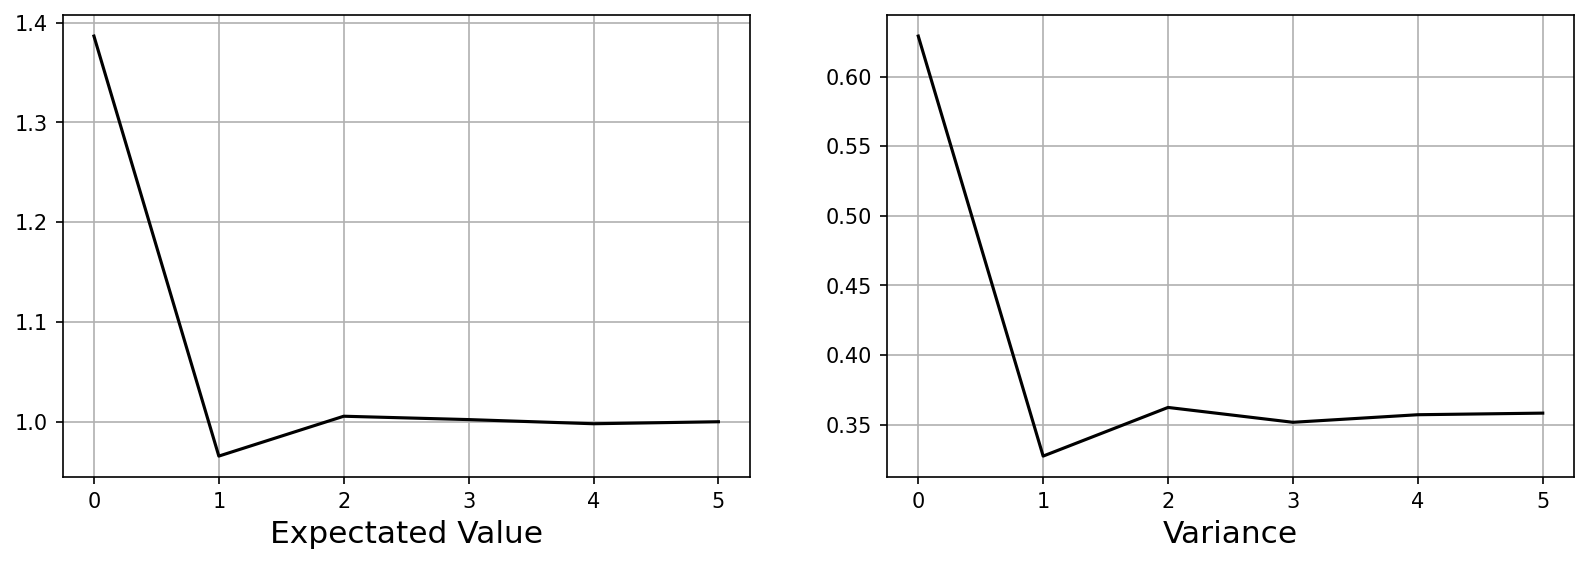
\includegraphics[width=0.8\textwidth]{int_h(x)_ipsam.png}
		\caption{Evaluating $\int_{0}^{10} e^{-2 |x-5|} dx$ using Importance Sampling.}
		\label{fig:impotrancesampling1}
	\end{figure}
	\begin{table}[h]
		\centering
		\begin{tabular}{lcc}
			\hline
			\textbf{Sample Size} & \textbf{Estimated Value (I=0.9999)} & \textbf{Variance} \\
			\hline
			10                   & 1.2473                              & 0.3812            \\
			100                  & 0.9292                              & 0.2593            \\
			1000                 & 1.0018                              & 0.3550            \\
			10000                & 1.0072                              & 0.3603            \\
			100000               & 1.0039                              & 0.3595            \\
			1000000              & 0.9999                              & 0.3580            \\
			\hline
		\end{tabular}
		\caption{Evaluating $\int_{0}^{10} e^{-2 |x-5|} dx$ using Importance Sampling.}
		\label{tab:mytable}
	\end{table}
	Here we can see that the estimation of $I$ is pretty close and variance is also
	lower the Original Monte Carlo method.
\end{example}

A more contemporary view of importance sampling is that we do not approach
importance sampling as an optimization problem, but because the circumstances
force us to consider different sampling distributions $F$.

Now, we also assume that $F_0,$ $F_1$ both have densities, say $f_0$, $f_1$.
If $F_0$, $F_1$ are both discrete then the notation only change but the argument is same.
Suppose then $f_i(x)=\frac{h_i(x)}{c_i},\ i=0,1$, where the assumption is that $h_0$, $h_1$
are completely known and also computable, but $c_0$, $c_1$ are unknown and are not even computable.
Then, as we showed above, for any function $\phi$ for which the expectation $E_{F_0}[\phi(X)]$ exist,

\begin{align*}
	\mu & = E_{F_0}[\phi(X)] := \int \frac{f_0(x)}{f_1(x)}\phi(x)f_1(x)dx      \\
	    & =\frac{c_1}{c_0} \int \frac{\phi(x)h_0(x)}{h_1(x)}f_1(x)dx           \\
	    & =\frac{c_1}{c_0} E_{F_1}\left( \frac{\phi(X)h_0(X)}{h_1(X)} \right).
\end{align*}

This is a useful reduction, but we have to deal with the fact that ratio $\frac{c_1}{c_0}$
is not known to us. Now, if we use the special function $\phi(x)\equiv 1$, the same
representation above gives us
\begin{align*}
	1                        & = \frac{c_1}{c_0} E_{F_1} \left( \frac{h_0(X)}{h_1(X)} \right) \\
	\implies \frac{c_1}{c_0} & = \frac{1}{E_{F_1} \left( \frac{h_0(X)}{h_1(X)} \right)}
\end{align*}
and because $h_0,$ $h_1$ are explicitly known to us, we have a way to get rid of the
quotient $\frac{c_1}{c_0}$ and write the final \textit{importance sampling identity}
\begin{align*}
	E_{F_0}[\phi(x)] = \frac{E_{F_1}\left( \frac{\phi(X)h_0(X)}{h_1(X)} \right)}{E_{F_1} \left( \frac{h_0(X)}{h_1(X)} \right)}
\end{align*}
We can now use an available Monte Carlo sample $X_1,X_2,\ldots,X_n$ from $F_1$
to find Monte Carlo estimates for $\mu = E_{F_0}[\phi(x)]$

The basic plug-in estimate for $\mu$ is the so-called ratio estimate
\[
	\hat{\mu} = \frac{\sum_{i = 1}^{n}\frac{\phi(X_i)h_0(X_i)}{h_1(X_i)} }{\sum_{i = 1}^{n} \frac{h_0(X_i)}{h_1(X_i)}}.
\]

\begin{example}[Binomial Bayes problem with an Atypical Prior]
	Suppose $X\sim Bin(m,p)$ for some fixed $m$ and $p$ has the prior density $c\sin^{2}(\pi p)$,
	where $c$ is a normalizing constant.
	Throughout the example, $c$ denotes a generic constant,
	and is not intended to mean the same constant at every use.

    The posterior density of $p$ given $X = x$ is
    \[
        \pi(p|X=x) = cp^{x}(1-p)^{m-x}\sin ^{2}(\pi p), \ \ 0<p<1.  
    \]
    The problem is to find the posterior mean
    \[
        \mu = c \int_{0}^{1} p[cp^{x}(1-p)^{m-x}\sin ^{2}(\pi p)]dp.
    \]

    We use importance sampling to approximate the value of $\mu$. Towards this, choose
    \[
        \phi(p)=p, \ h_0(p) = p^{x} (1-p)^{m-x} \sin ^{2}(\pi p),\ h_1(p) = p^{x}(1-p)^{m-x},   
    \]
    so that if $p_1,p_2,\ldots,p_n$ are samples from $F_1$, (i.e. $p_i\sim Beta(x+1, m-x+1)$),
    then the importance sampling estimate of the posterior mean $\mu$ is
    \begin{align*}
        \hat{\mu} &= \frac{\sum_{i=1}^{n}\frac{\phi(p_i)h_0(p_i)}{h_1(p_i)} }{\sum_{i=1}^{n}\frac{h_0(p_i)}{h_1(p_i)} } \\ 
                  &= \frac{\sum_{i=1}^{n}p_i\sin ^{2}(\pi p_i) }{\sum_{i=1}^{n} \sin ^{2}(\pi p_i) }.
    \end{align*}

    Note that we did not need to calculate the normalizing constant in the posterior density.
    We take $m=100$, $x=45$ for specificity.

\end{example}
